\documentclass{article}
\usepackage{graphicx}
\usepackage[position=top]{subfig}
\usepackage[left=1in,right=1in,top=1in,bottom=1in]{geometry}
 \usepackage{pxfonts}


 \newcommand{\familiarity}{2}



\begin{document}

\title{Supporting Materials for \textit{Category-based and location-based volitional covert attention affect
memory at different timescales}}

\author{Kirsten Ziman\textsuperscript{$1, 2$},
Madeline R. Lee$^1$,
Alejandro R. Martinez$^1$,\\
Ethan D. Adner$^1$,
and
Jeremy R. Manning\textsuperscript{$1, \dagger$}\\[0.1in]$^1$Dartmouth College\\
$^2$Princeton University\\
\textsuperscript{$\dagger$}Address correspondence to jeremy.r.manning@dartmouth.edu}


\maketitle


\renewcommand{\thefigure}{S\arabic{figure}}


  \begin{figure*}[tp]
	\centering
	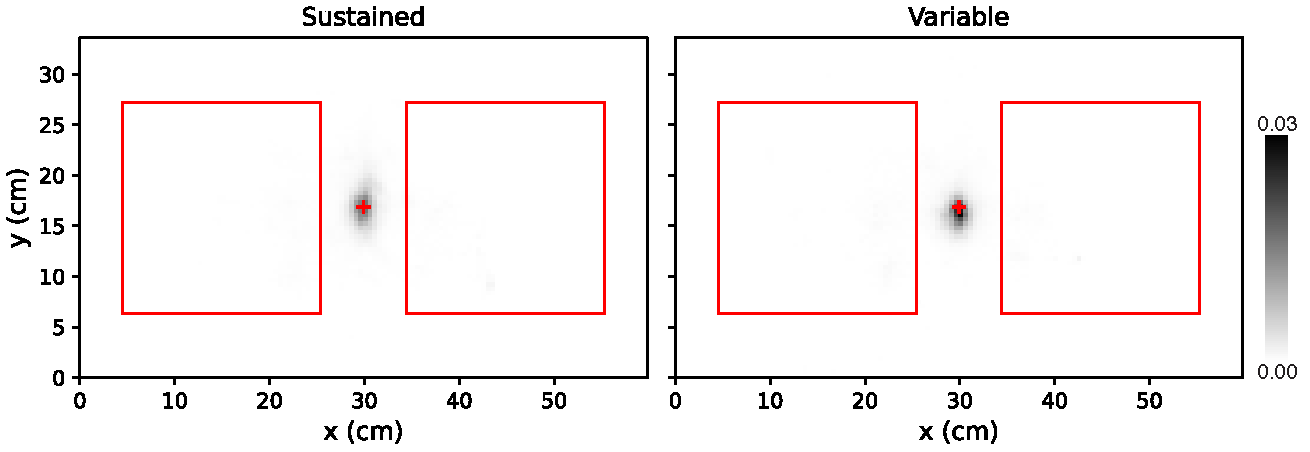
\includegraphics[width=1\textwidth]{figs/gaze_locations}
  
 \caption{\textbf{Gaze location histograms.} We divided the experimental
 display into 120 horizontal bins and 78 vertical bins, each comprising a
 roughly 0.5~cm square. The panels display the average proportions of time
 (throughout the duration of the experiment) participants spend looking at each
 location. The left panel displays data from participants in the sustained
 attention condition and the right panel displays data from participants in the
 variable attention condition. In both panels, the locations of the central
 fixation cross (red $+$) and composite images (red-outlined squares) are
 indicated.}
  
  \label{fig:gaze-histograms}
  \end{figure*}

  \begin{figure*}[tp]
	\centering
	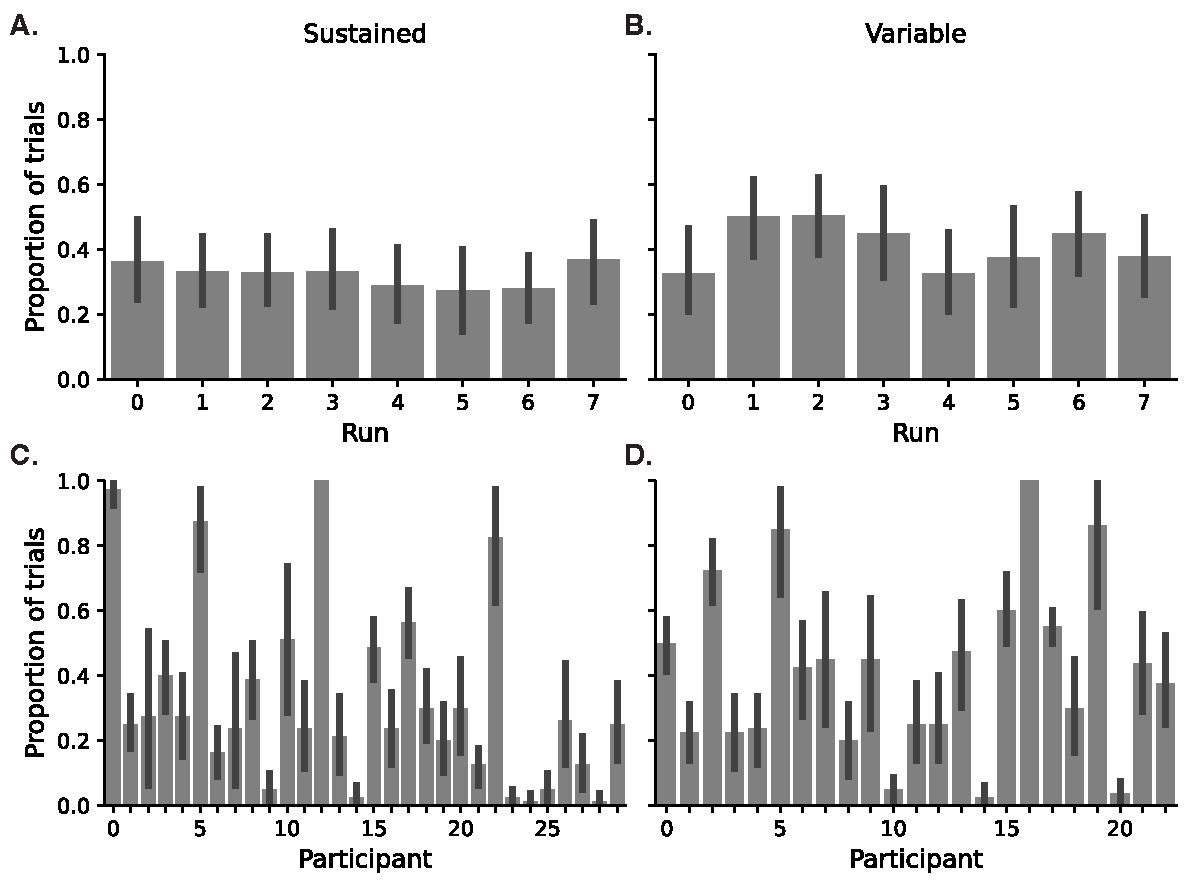
\includegraphics[width=1\textwidth]{figs/gaze_intersections}
  
\caption{\textbf{Proportions of excluded trials.} We excluded from our analyses
any images from trials where the participant's gaze touched on any part of the
attended composite image (attended-side red squares in
Fig.~\ref{fig:gaze-histograms}). \textbf{A--B. Proportions of excluded trials,
by run.} Across both experimental conditions (left: sustained attention; right:
variable attention), the bars display the average proportions of presentations
from each run where participants looked at any part of the attended composite
image, for any non-zero duration. Error bars denote across-participant
bootstrap-estimated 95\% confidence intervals. \textbf{C--D. Proportions of
excluded trials, by participant.} Across both experimental conditions (left:
sustained attention; right: variable attention), the bars display the average
proportions of presentations across different runs where the given
pariticapants looked at any part of the attended composite image, for any
non-zero duration. Error bars denote across-run bootstrap-estimated 95\%
confidence intervals.}

  \label{fig:gaze-histograms}
\end{figure*}

\begin{figure*}[tp]
  \centering
  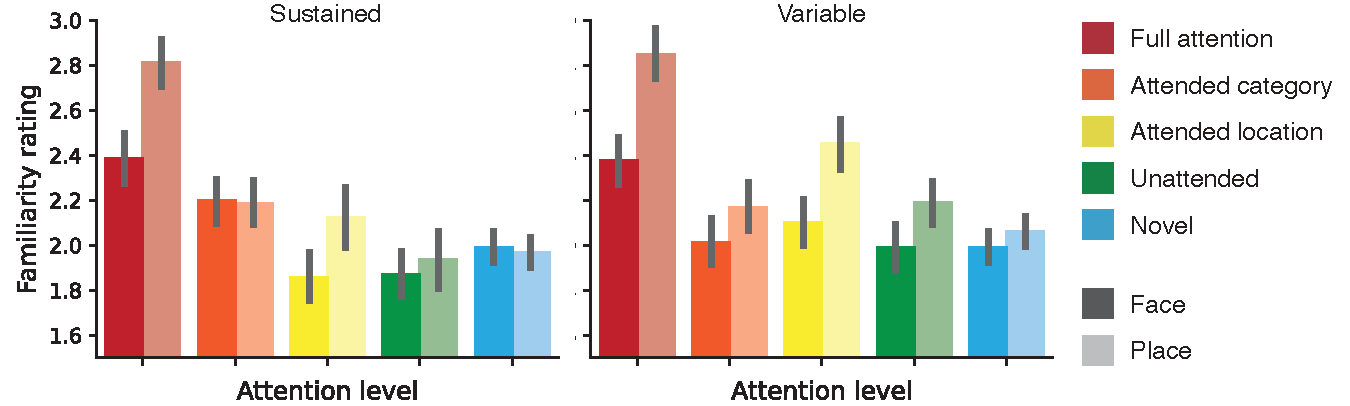
\includegraphics[width=1\textwidth]{figs/familiarity_by_attention_level and_category}

\caption{\textbf{Familiarity by attention level and stimulus category.} The
bars display the average familiarity ratings participants gave to images from
the same category and location as the attention cue (fully attended), the same
category (but opposite location) as the attention cue (attended category), the
same location (but opposite category) as the attention cue (attended location),
the opposite category and location as the attention cue (unattended), or novel
images. Each family of bars is further sub-divided according to whether the
rated stimulus was a face (darker shading) or a place (lighter shading) image.
The left panel displays familiarity ratings from the sustained attention
condition and the right panel displays familiarity ratings from the variable
attention condition. All error bars denote across-participant
bootstrap-estimated 95\% confidence intervals. Also see Figure~\familiarity~in
the main text.}

\label{fig:ratings-by-category}
\end{figure*}


\begin{figure*}[tp]
  \centering
  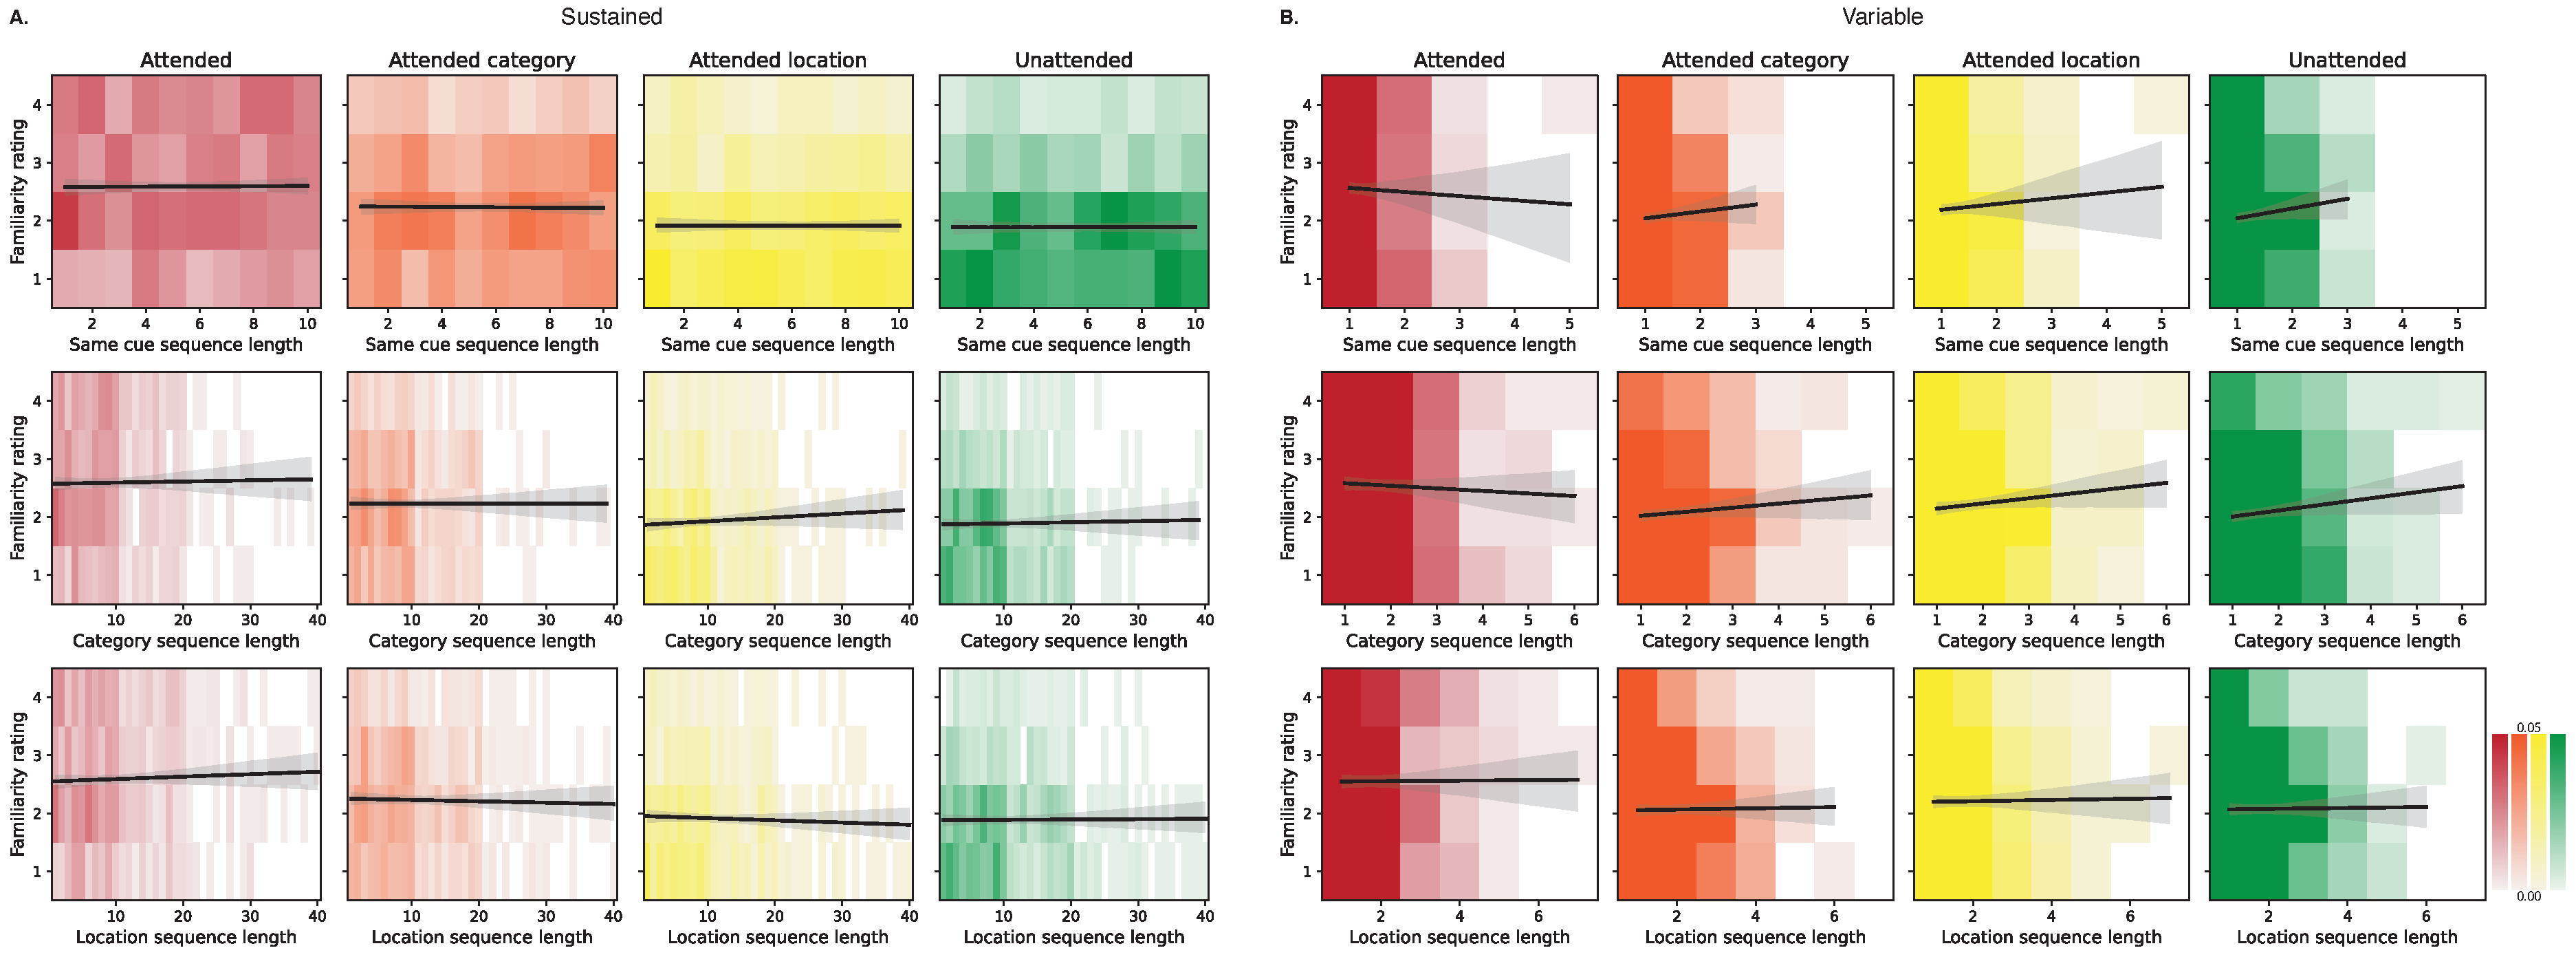
\includegraphics[width=1\textwidth]{figs/sequence_length_effects}

\caption{\textbf{Effects of attention cue sequence length on familiarity.} 
\textbf{A. Sequence effects (sustained attention condition).} Each heatmap
displays the proportions of images that participants rated at each familiarity
rating (rows), broken down by the number of successive matching attention cues
the participant received at the time the given image was presented as part of a
composite pair (up to and including the image's composite pair; columns). The
trend lines (with bootstrap-estimated 95\% confidence intervals) show
regressions fit to the corresponding heatmap's data ($x$: sequence length; $y$:
familiarity rating). Heatmaps are organized into rows based on how the sequence
lengths were computed (top row: successive attention cues had the same category
and location; middle row: successive attention cues had the same category;
bottom row: successive attention cues had the same location). Columns (and
colors) denote attention levels (as in Figs.~\familiarity~and
\ref{fig:ratings-by-category}). \textbf{B. Sequence effects (variable attention
condition).} This Panel is in the same format as Panel A, but displays results
from the variable attention condition.}

\label{fig:sequence-effects}
\end{figure*}

\begin{figure*}[tp]
  \centering
  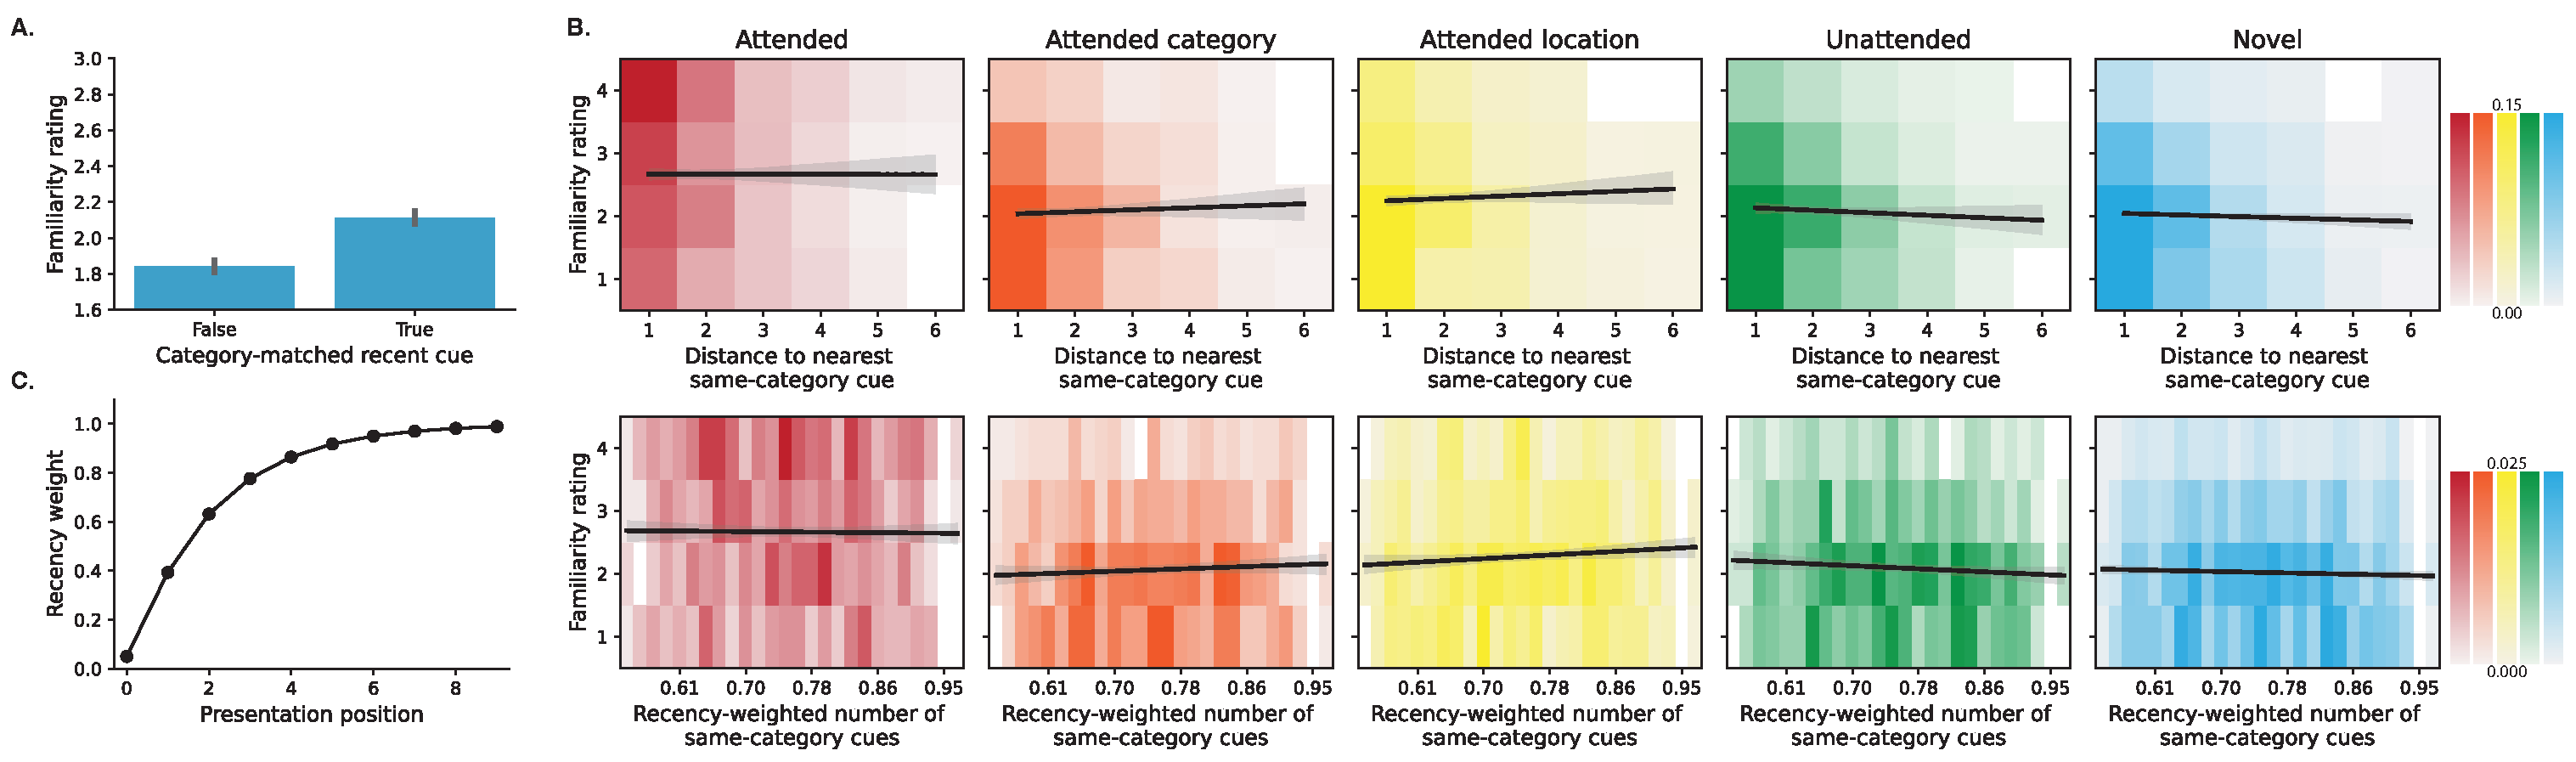
\includegraphics[width=1\textwidth]{figs/response_bias.pdf}

\caption{\textbf{Response bias analyses.} \textbf{A. Sustained attention
condition.} The bars display the mean familiarity ratings participants gave to
novel memory probes (lures) that matched (``True'') versus did not match
(``False'') the prior run's attention-cued category. Error bars denote
across-participant bootstrap-estimated 95\% confidence intervals. \textbf{B.
Variable attention condition.} Each heatmap displays the proportions of images
that participants rated at each familiarity rating (rows), broken down by
metrics related to recent same-category attention cues participants received on
the prior run (columns). The trend lines (with bootstrap-estimated 95\%
confidence intervals) show regressions fit to the corresponding heatmap's data
($x$: metrics related to same-category cues; $y$: familiarity rating). The top
panels's columns reflect the temporal distances to the most recent
same-category attention cues, measured in numbers of presented items (where 1
denotes the final item on the most recent run). The bottom panel's columns
denote the recency-weighted average numbers of same-category cues presented on
the most recent run. Each column of matrices corresponds to a different
attention level, as in Figures~\familiarity~and \ref{fig:ratings-by-category}.
\textbf{C. Weights by recency.} The panel displays the weights used to compute
recency-weighted numbers of same-category cues on the most recent run. The
$x$-axis displays the presentation positions of each attention cue, and the
$y$-axis displays the weight assigned to same-category cues at the given
presentation position. The weights are first computed using $w = \max\left[1 -
\exp\{-\frac{x}{\tau}\} , \epsilon \right]$, where $\tau = 2$, $\epsilon =
0.05$, and $x$ is the cue's presentation position. To obtain the $y$-values
shown in the Panel (and used in Panel B), the weights for $x \in \left[0, 1, 2,
..., 9\right]$ are normalized to sum to 1.}

\label{fig:response-bias}
\end{figure*}




\end{document}
